\documentclass{beamer} %[12pt]
\usepackage{xcolor}
%\usetheme{boadilla}
%\usetheme{malmoe}
%\usetheme{copenhagen}
%\usecolortheme{rose}
\usecolortheme{beaver}
\usepackage{pgf, graphics}
\usepackage{graphicx}
%\usepackage[left=3cm,top=3cm,right=3cm,nohead,nofoot]{geometry}
\usepackage{hyperref}
\usepackage{setspace}
\usepackage[square]{natbib}
\usepackage{amsmath}
\usepackage{amssymb}
\usepackage{verbatim}
\usepackage{color}
\usepackage{fancyvrb}
\usepackage{bbm}

\begin{filecontents}{ref.bib}
\end{filecontents}

%\usetheme{EastLansing}
%\usepackage{natbib}
\bibliographystyle{apalike}
% make bibliography entries smaller
%\renewcommand\bibfont{\scriptsize}
% If you have more than one page of references, you want to tell beamer
% to put the continuation section label from the second slide onwards
\setbeamertemplate{frametitle continuation}[from second]
% Now get rid of all the colours
\setbeamercolor*{bibliography entry title}{fg=black}
\setbeamercolor*{bibliography entry author}{fg=black}
\setbeamercolor*{bibliography entry location}{fg=black}
\setbeamercolor*{bibliography entry note}{fg=black}
% and kill the abominable icon
\setbeamertemplate{bibliography item}{}


\newcommand{\hl}[1]{\colorbox{yellow}{#1}}
\newcommand{\hlblue}[1]{\colorbox{green}{#1}}
\newcommand{\hlblu}[1]{\colorbox{cyan}{#1}}
\newcommand{\hlred}[1]{\colorbox{cyan}{#1}}
\newcommand{\hlre}[1]{\colorbox{pink}{#1}}
\newcommand{\hlgreen}[1]{\colorbox{pink}{#1}}
\newcommand{\hlgree}[1]{\colorbox{green}{#1}}



\DeclareMathOperator*{\argmax}{\arg\!\max}

\DeclareMathOperator*{\argmin}{\arg\!\min}


\newcommand{\specialcell}[2][c]{%
  \begin{tabular}[#1]{@{}c@{}}#2\end{tabular}}



%\setbeamersize{text margin left=.5cm,text margin right=.5cm}
\newenvironment{changemargin}[2]{%
  \begin{list}{}{%
    \setlength{\topsep}{0pt}%
    \setlength{\leftmargin}{#1}%
    \setlength{\rightmargin}{#2}%
    \setlength{\listparindent}{\parindent}%
    \setlength{\itemindent}{\parindent}%
    \setlength{\parsep}{\parskip}%
  }%
  \item[]}{\end{list}}
\setbeamertemplate{navigation symbols}{}%remove navigation symbols
\usepackage{color}
\newcommand{\hilight}[1]{\colorbox{yellow}{#1}}
\setbeamertemplate{footline}[page number]

\begin{document}


\title[dedup]{Today:  Maps}


\author[Samuel L. Ventura]{\\
  \large{Sam Ventura\\36-315\\Today:  Maps}}
\institute[CMU Statistics]{Department of Statistics\\Carnegie Mellon University}
\date{\today}


\begin{frame}
	\maketitle

	
\end{frame}




\begin{frame}\frametitle{Earliest Graphics}
	\centering
	Began with geographic maps:  \\symbols/colors on clay tablets (5000 years ago)
	
	\vskip 0.5 cm
	
	11th century China:  Map of the Tracks of Yu The Great\\coastal outline very accurate\\high precision of rivers\\scale is almost exact\\carved into 3-ft wide stone tablet
	
\end{frame}



\begin{frame}\frametitle{Map of the Tracks of Yu The Great}
	\centering
	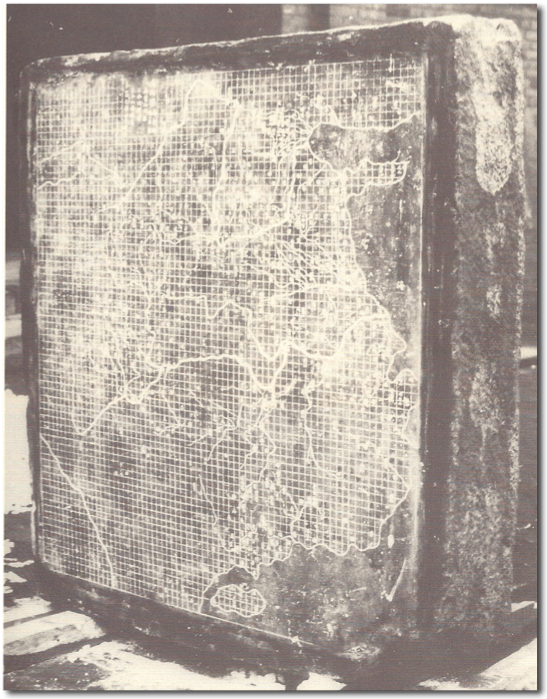
\includegraphics[width=0.6\linewidth]{yu2.png}
\end{frame}



\begin{frame}\frametitle{Map of the Tracks of Yu The Great}
	\centering
	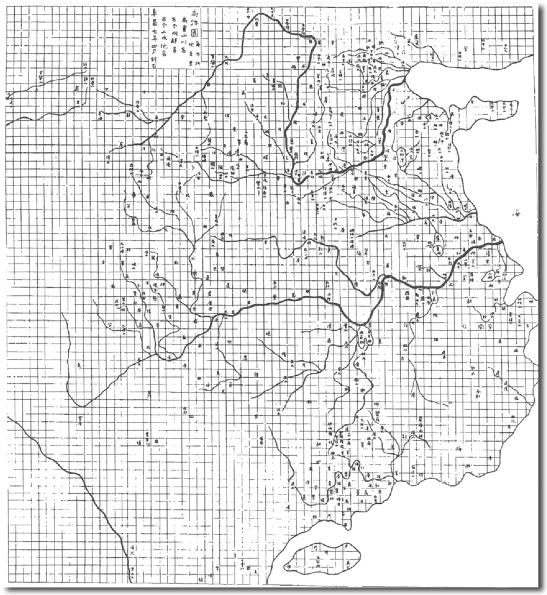
\includegraphics[width=0.7\linewidth]{yu.png}
\end{frame}




\begin{frame}\frametitle{La Verdadera Longitud por Mar y Toledo}
	\centering
	Shows statistical information!
	
	\vskip 1 cm
	
	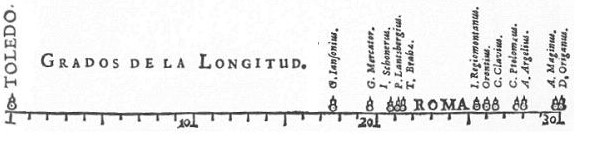
\includegraphics[width=\linewidth]{longitud.jpg}
	
	\vskip 1 cm
	
	Wide range of estimates of distance from Rome to Toledo
\end{frame}



\begin{frame}\frametitle{Minard -- Exports of French Wine}
	\centering
	\includegraphics[width=\linewidth]{trade.jpg}
\end{frame}


\begin{frame}\frametitle{Cholera Mapping}
	\centering
	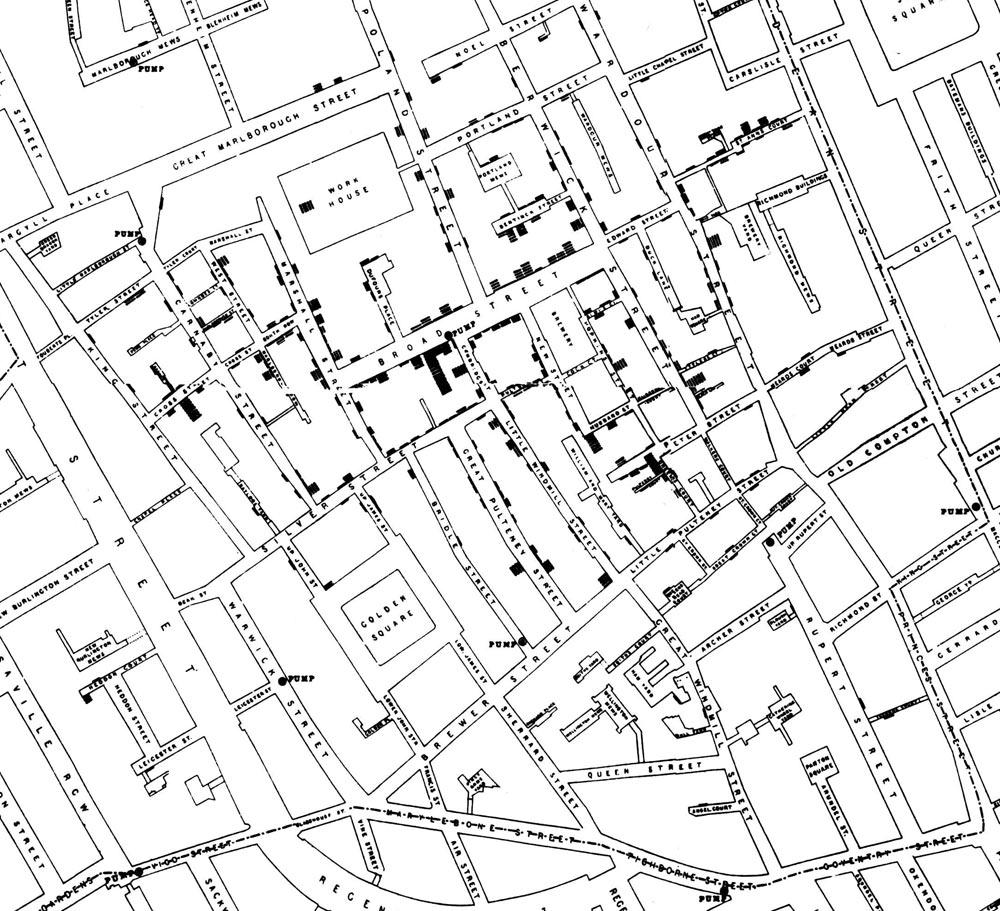
\includegraphics[width=0.8\linewidth]{cholera.jpg}
\end{frame}


\begin{frame}\frametitle{Napolean's March To Moscow}
	\centering
	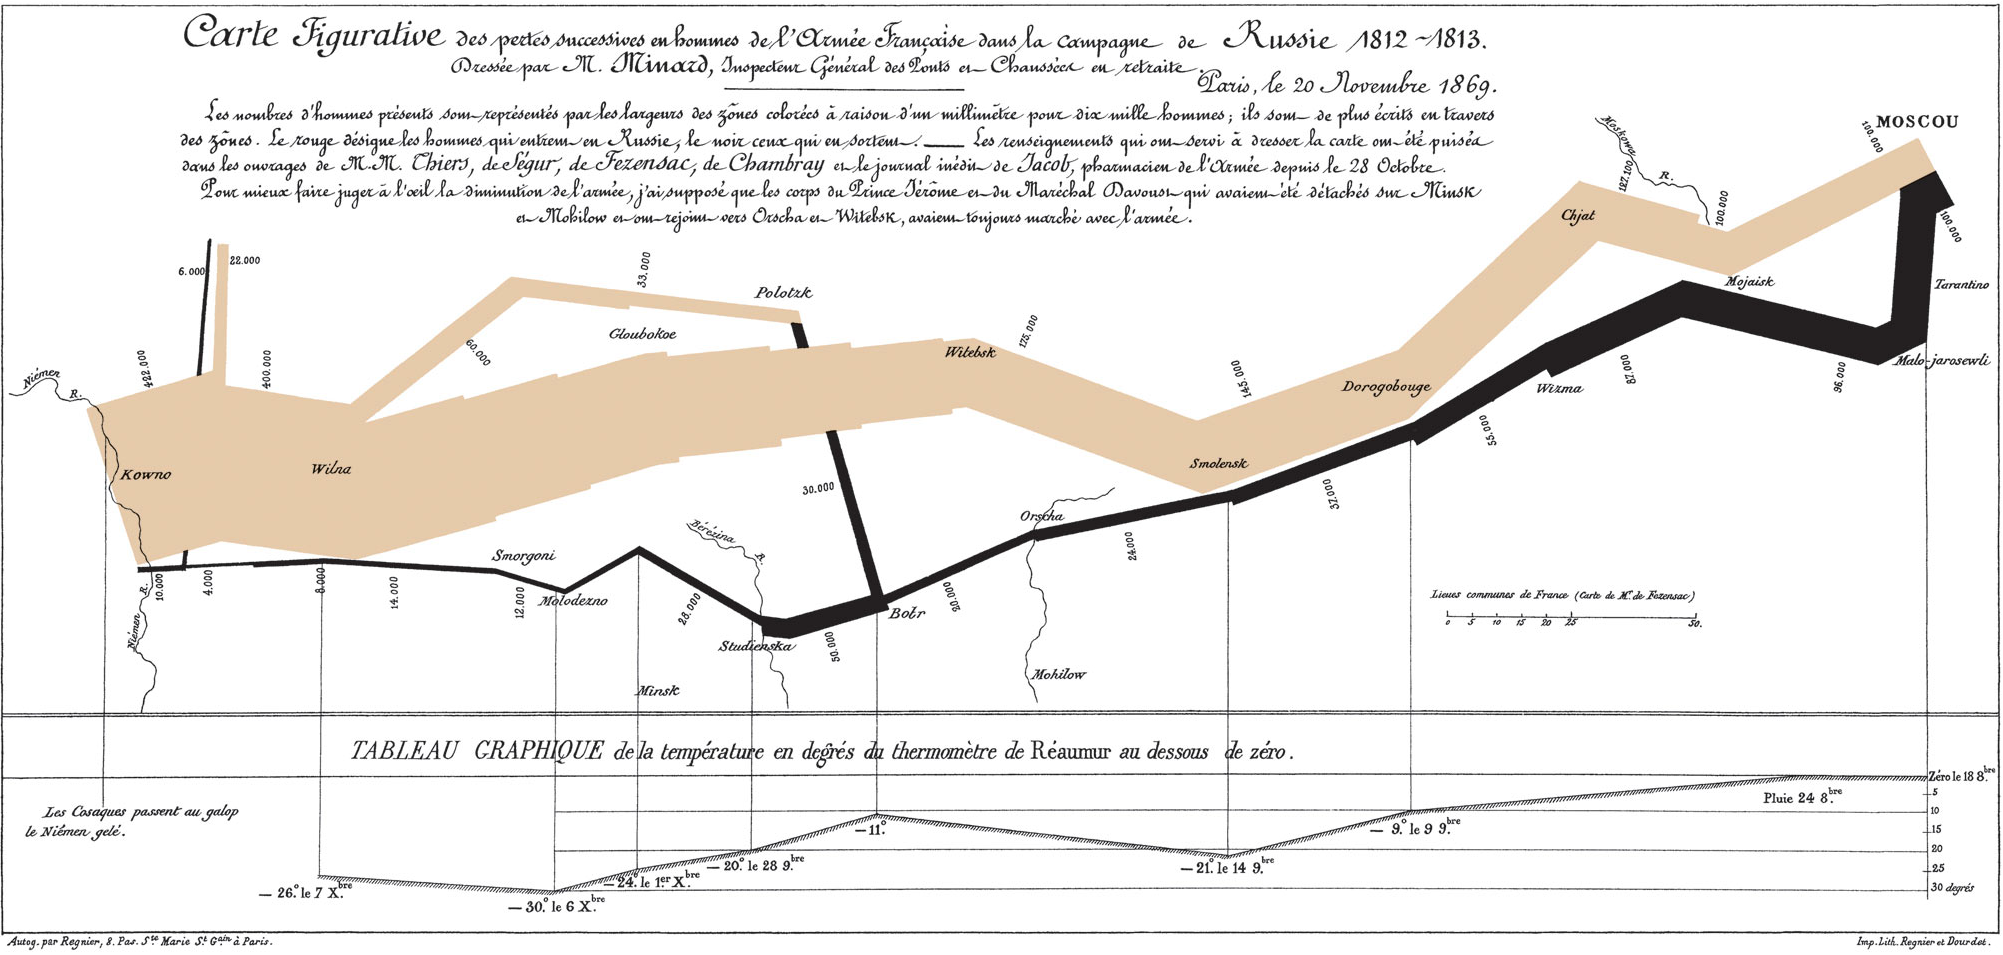
\includegraphics[width=\linewidth]{Minard.png}
	
	%  This map drawn by Charles Joseph Minard portrays thelosses suffered by Napoleon's army in the Russian campaign of 1812. Beginning at the left on the Polish-Russian border near the Niemen, the thick band shows the size of hte army (422K men) as it invaded Russia.  The width of the band indicates the size of the army at each position.  In september, the army reached Moscow with 100,000 men.  The path of Napoleon's retreat from Moscow in the bitterly cold winter is depicted by the dark lower band, which is tied to temperature and time scales.  The remains of the Grande Armee struggled out of Russia with 10,000 men.  Minard's graphic tells a rich, coherent story with its multivariate data, far more enlightening than just a single number bounching along over time.  Six variables are plotted:  The size of the army, its location on a two-dimensional surface, direction of the army's movement, and temperature on various dates during the retreat from Moscow.  It may well be the best statistical graphic ever drawn.  
\end{frame}



\begin{frame}\frametitle{Hourly Wages to Afford Two-Bedroom Apartment}
	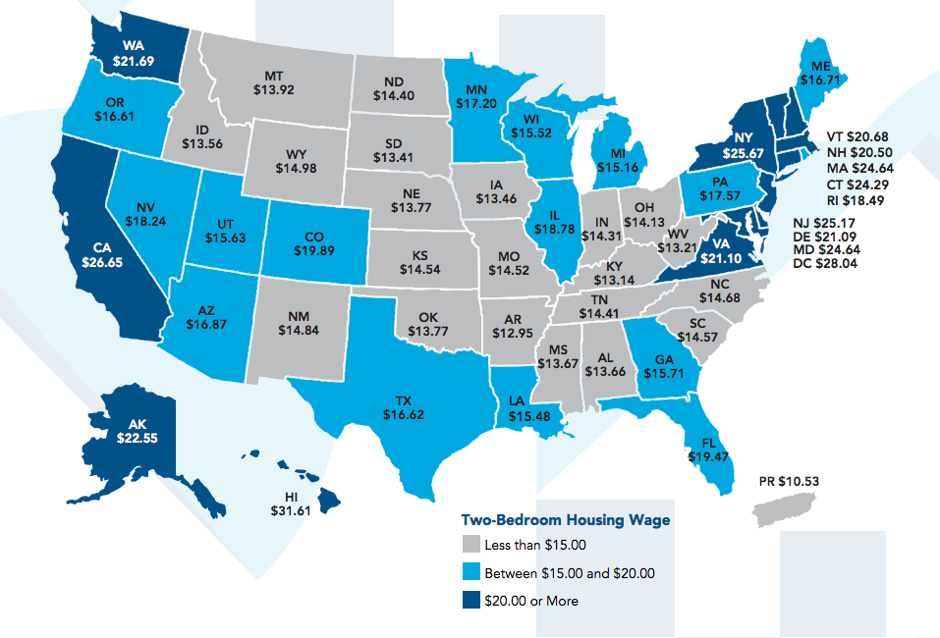
\includegraphics[width=\linewidth]{hourly.png}
\end{frame}



\begin{frame}\frametitle{US Income by Census Tract}
	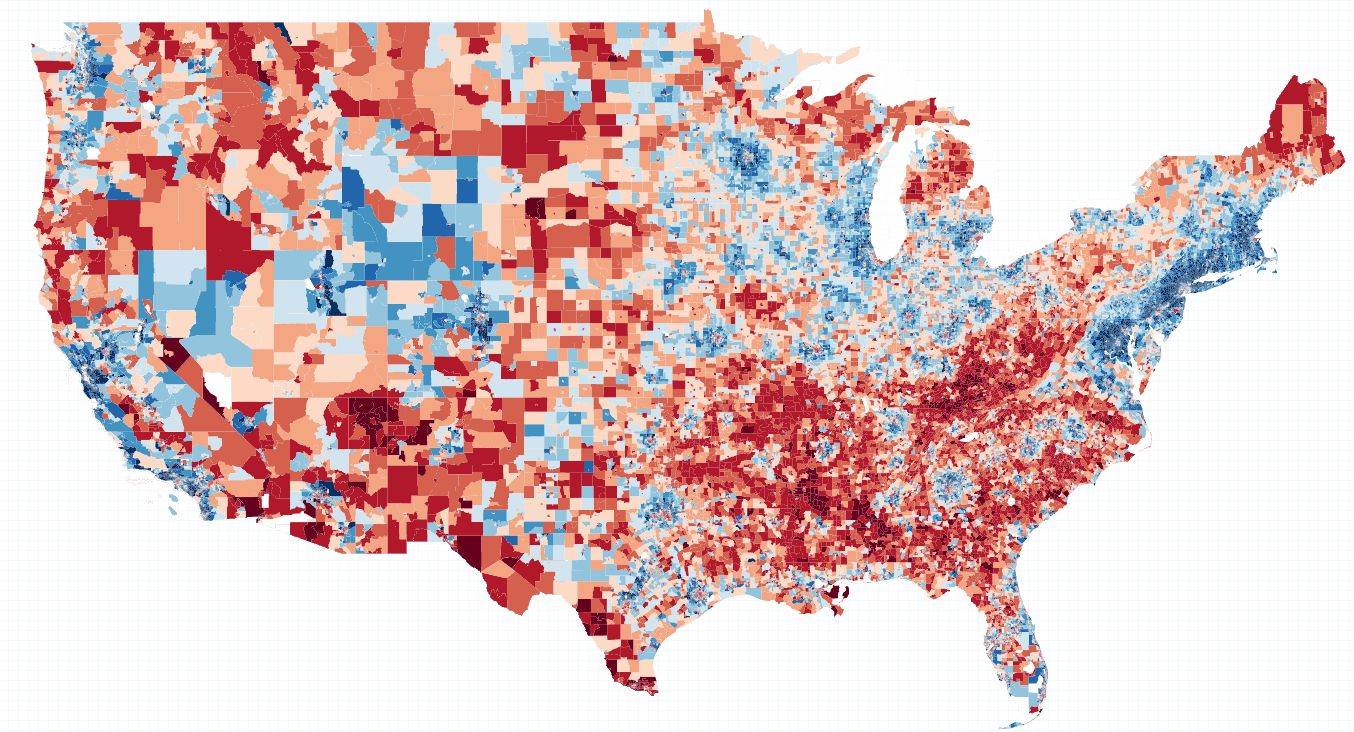
\includegraphics[width=\linewidth]{income-tract.jpg}
\end{frame}



\begin{frame}\frametitle{Maps}
	\small
	
	\textbf{Latitude and Longitude:}  
	%  Latitude measures distance from equator (north/south; "y-axis")

	%  Measured in degrees, from -90 to 90
	
	%  Longitude measures distance from prime meridian (east/west; "x-axis")
	
	%  Measured in degrees, from -180 to 180
	\vskip 3 cm
	
	%  Draw pictures of earth with latitude and longitude lines
	
	\vskip 10 cm
	
\end{frame}



\begin{frame}\frametitle{Map Projections}
	\small
	
	\textbf{Earth is a 3-D object, but maps are 2-D objects.}  
	%  Latitude measures distance from equator (north/south; "y-axis")
	
	%  Longitude measures distance from prime meridian (east/west; "x-axis")
	
	\vskip 0.5 cm
	
	\textbf{Map Projections:}  %  Systematic transformation of the latitudes and longitudes of locations on the surface of a sphere into locations on a (usually 2-D) plane.  Sound familiar?
	
	%  ALL map projections distort the surface of the sphere (Earth) in some way.
	
	%  Other applications of map projections:  Neuroscience!  Brain is sort of spherical / ellipsoidal, so can use similar techniques.
	
	\vskip 4 cm
	
	\textbf{Common Projections:}  %  Mercator, Robinson, Conic, Cylindrical, Plane, Interrupted, etc.
	
	\vskip 10 cm
	
\end{frame}



\begin{frame}\frametitle{Mercator Projection}
	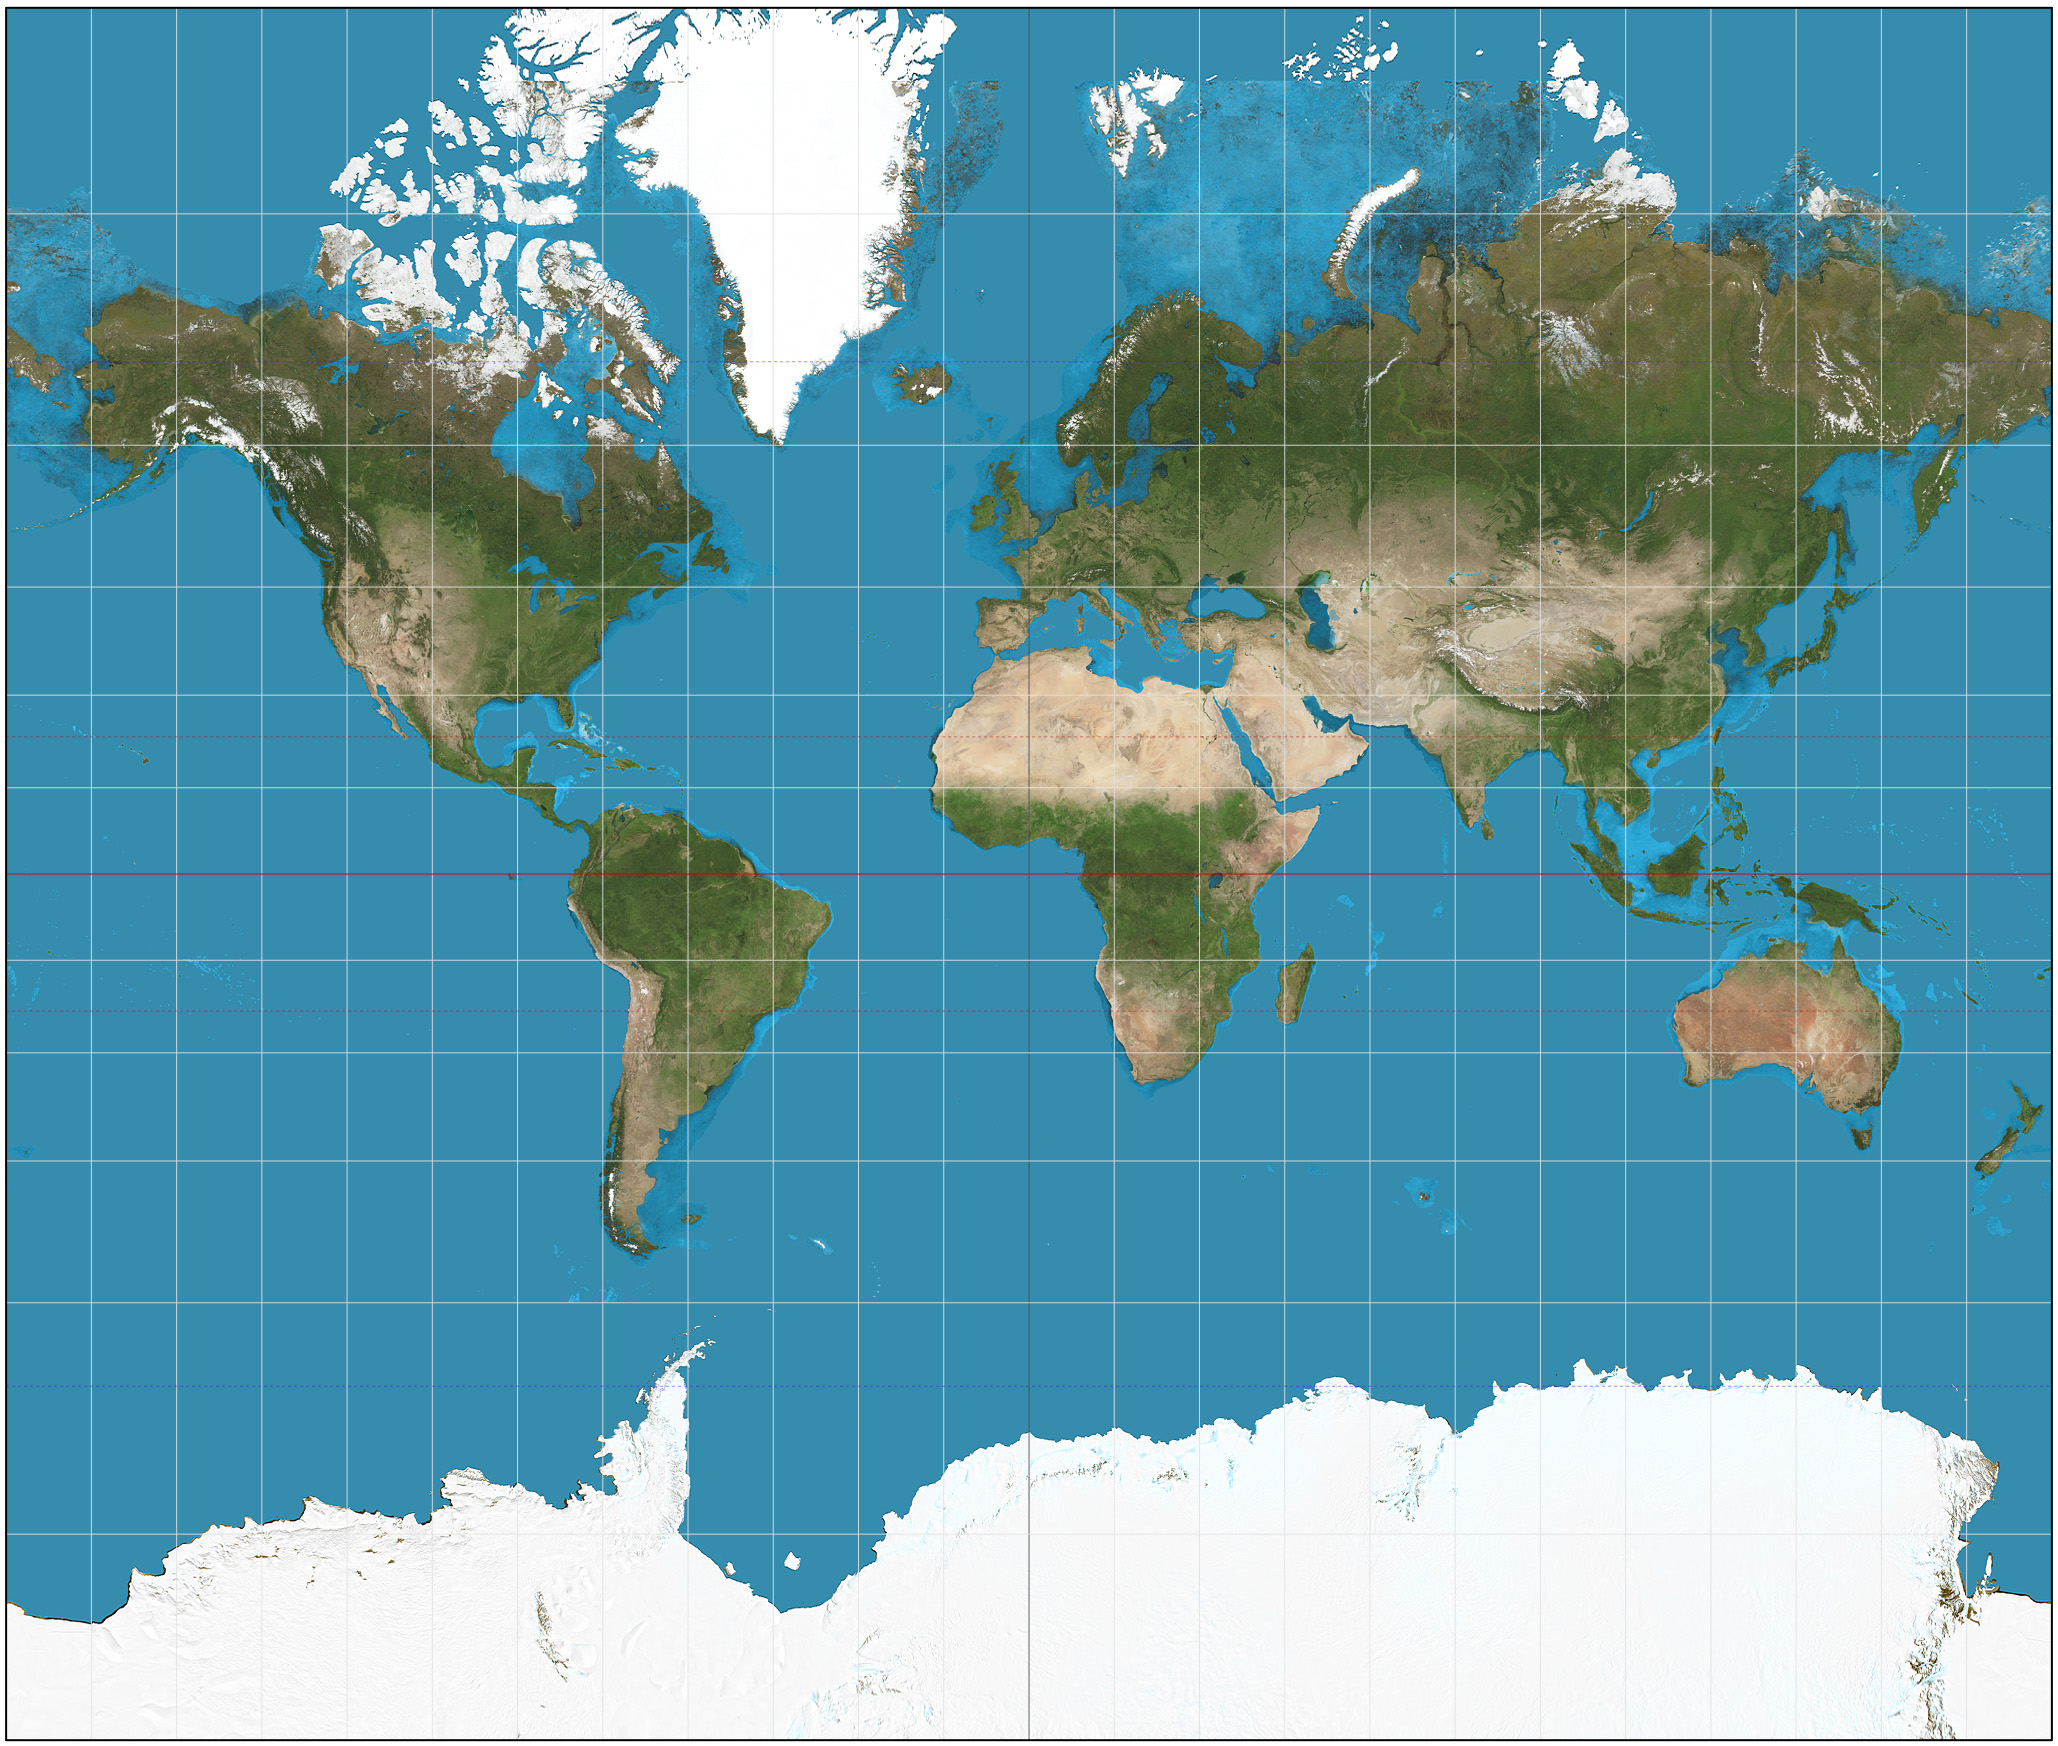
\includegraphics[width=0.9\linewidth]{mercator.jpg}
\end{frame}





\begin{frame}\frametitle{Mercator Projection}
	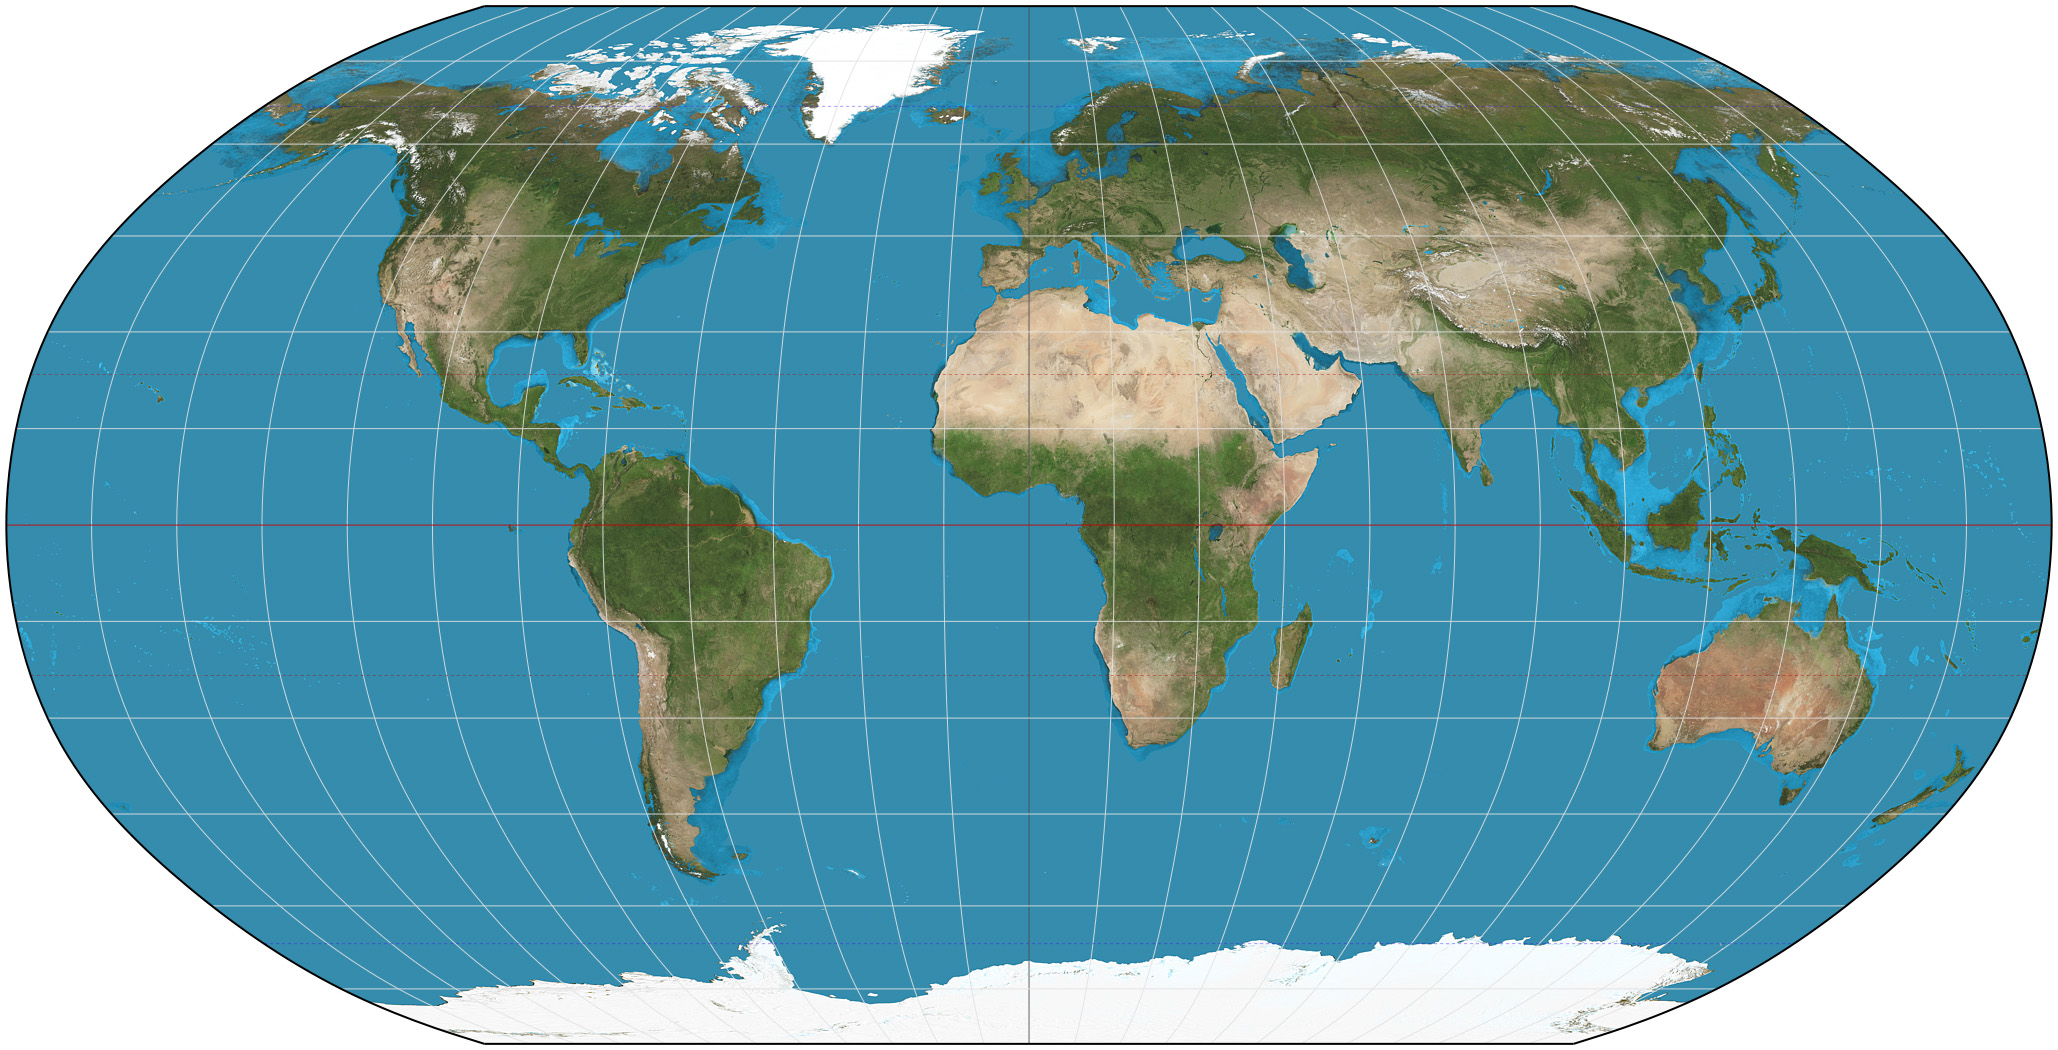
\includegraphics[width=\linewidth]{robinson.jpg}
\end{frame}





\begin{frame}\frametitle{More Projections}
	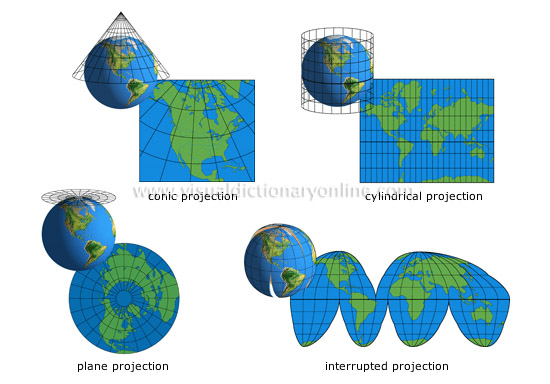
\includegraphics[width=\linewidth]{projections2.jpg}
\end{frame}





\begin{frame}\frametitle{US Projections}
	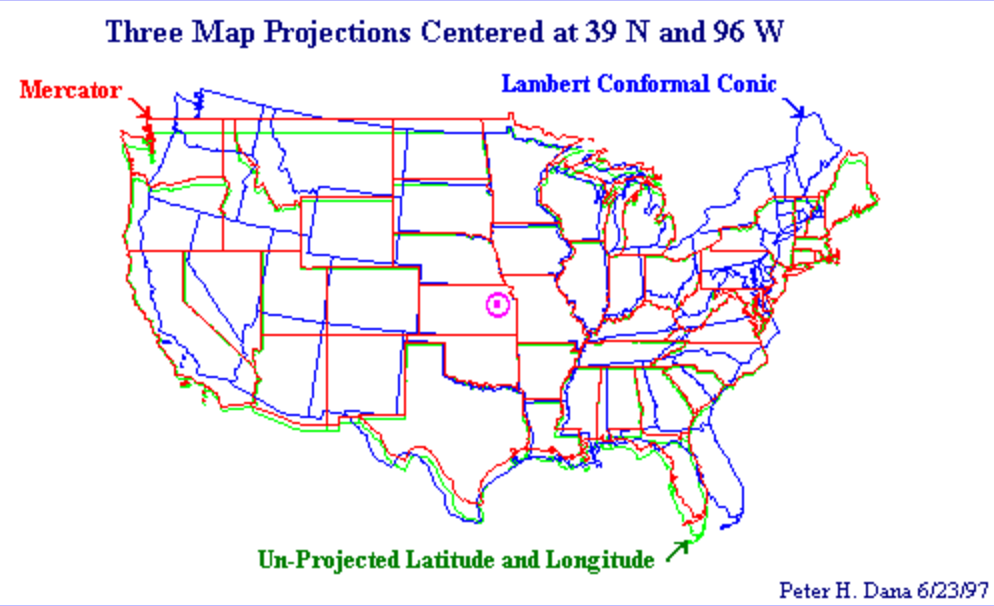
\includegraphics[width=\linewidth]{us.png}
\end{frame}





\begin{frame}\frametitle{Census Geographies}
	\small
	
	\centering
	
	\textbf{Geographic Hierarchy for Government Administrative Purposes}  %  Country, states, PUMAs/counties, tracts, block groups, blocks
	
	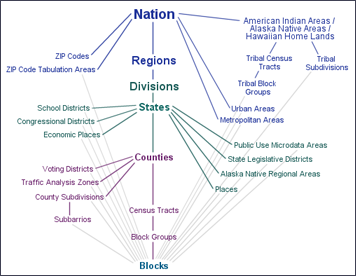
\includegraphics[width=0.8\linewidth]{census-geographic-hierarchy.png}
\end{frame}




\begin{frame}\frametitle{Maps in R (and other software/tools) with Shapefiles}
	\small
	
	\textbf{Shapefiles}:  
	
	%Data Objects that contain spatial polygons
	
	\vskip 4 cm
	
	%  Can contain points, lines, polygons representing any geographic feature
	
	%  Available for countries, states, counties, tracts.
	
	\vskip 10 cm
	
\end{frame}



\end{document}
